\chapter{Fundamentação Teórica}

Este capítulo apresenta uma breve introdução sobre os conceitos tocados neste
trabalho. Primeiro, é abordado as partes do \textit{pipeline} de um compilador
de maneira a entender, ao menos superficialmente, os passos de compilação.
Em seguida, discute-se conceitos de computação paralela e possíveis abordagens
de paralelismo.

\begin{section}{Compiladores}

Para evitar confusões a respeito das diferentes linguagens que um compilador
trabalha em seus muitos estágios, vamos adotar a seguinte nomenclatura. 

\textit{Definição.} Denote como \textit{Linguagem Fonte} como sendo a linguagem
na qual o código fonte foi originalmente escrito;
\textit{Linguagem Intermediária} as linguagens internas do compilador; e
\textit{Linguagem Alvo} a linguagem na qual o compilador deverá gerar código.


Compiladores são grandes projetos destinados a tradução de códigos fonte
entre distintas linguagens de programação. Normalmente, compiladores traduzem
linguagens de alto nível, como C, para linguagens mais próximas da máquina,
como a linguagem de montagem, embora isso não seja uma regra.
Compiladores também costumam otimizar
o código que passam por eles, aplicando diversas heurísticas de
maneira a acelerar o código a ser produzido, substituindo trechos de código por 
outros mais eficientes, reordenando as instruções do programa, etc.

Por serem programas extremamente grandes, existe um grande interesse em evitar
reescrever um novo compilador 
sempre que uma nova linguagem é proposta, ou um novo \textit{hardware} é criado.
Para isso, a seguinte modularização é largamente adotada por projetistas de
compiladores \citep{redhat} \citep{llvm}, conforme ilustrado na Figura \ref{fig:compiler_arch}:

\begin{itemize}
    \item Um \textit{Front End} para cada Linguagem Fonte a ser compilada. 
	É neste módulo que é executado a análise léxica e sintática para a
construção da a Árvore de Sintaxe Abstrata (AST), para que em
seguida ela seja convertida para uma Linguagem Intermediária do compilador.

    \item Um \textit{Middle End}, responsável por aplicar diversas otimizações
independentes de arquitetura no código já convertido para a Linguagem Intermediária.

    \item Um \textit{Back End} para cada linguagem alvo, responsável por converter a linguagem intermediária
na linguagem alvo. Aqui outras otimizações específicas da linguagem alvo são realizadas,
como alocação de registradores, e o código é finalmente convertido para a linguagem alvo.

\end{itemize}

Porém, essa modularização é opcional: compiladores mais antigos destinados a fazer uma
conversão direta entre duas linguagens como o UNIX C Compiler  não costumam usar uma linguagem
intermediária \citep{ritchie1979tour}, além de diversos livros-texto não mencionarem tal módulo, fundindo suas
funcionalidades com o \textit{Front End} \citep{dragonbook}. Não adotar tal metodologia
simplifica o projeto, mas dificulta a inserção de suporte à novas
linguagens de programação. 


\begin{figure}
\tikzstyle{block} = [rectangle, draw, fill=white,
    text width=6em, text centered, rounded corners, node distance=5cm, auto, minimum height=2em]
\tikzstyle{line} = [draw, -latex]
\tikzstyle{cloud} = [draw, ellipse,fill=white, node distance=2cm,
    minimum height=2em]

\begin{center}
\scalebox{0.8}{
\begin{tikzpicture}[node distance = 3cm, auto]
    % Place nodes
    \node [block]                      (front_c)    {Frontend C};
    \node [block, below of=front_c]    (front_cpp)  {Frontend C++};
    \node [block, below of=front_cpp]  (front_fort) {Frontend Fortran};
    \node [block, right of=front_cpp]  (middle)     {Middle End};
    \node [block, right of=middle]     (back_x86)   {Backend x86};
    \node [block, above of=back_x86]   (back_arm)   {Backend ARM};
    \node [block, below of=back_x86]   (back_ppc)   {Backend PPC};


    \coordinate [left of=front_c]    (c_code);
    \coordinate [left of=front_cpp]  (cpp_code);
    \coordinate [left of=front_fort]  (fort_code);

    \coordinate [right of=back_x86] (x86_code);
    \coordinate [right of=back_arm] (arm_code);
    \coordinate [right of=back_ppc] (ppc_code);

    % Draw edges
    \draw[->]    (front_c.east)     to [out=0,in=180] ([yshift=0.5em]  middle.west);
    \draw[->]    (front_cpp.east)   to [out=0,in=180] (middle.west);
    \draw[->]    (front_fort.east)  to [out=0,in=180] ([yshift=-0.5em] middle.west);

    \draw[->]    ([yshift=-0.5em] middle.east)  to [out=0,in=180] (back_ppc.west);
    \draw[->]    (middle.east)                  to [out=0,in=180] (back_x86.west);
    \draw[->]    ([yshift=0.5em] middle.east)   to [out=0,in=180] (back_arm.west);

    %\draw[->]    (sintatico.west)   -- (lexico.east)    node[midway] {próximo\_token()};
    %\draw[->]    (fonte.west)       -- (lexico.west)    node[pos=0, above] {Código Fonte};
    %\draw[->]    (sintatico.east)   -- (ast.west)       node[pos=1, above] {Árvore Abstrata};
\end{tikzpicture}
}
\end{center}

\caption{Arquitetura de um compilador.}
\label{fig:compiler_arch}
\end{figure}

\begin{subsection}{\textit{Front End}}

Um \textit{Front End} é o módulo responsável por interagir diretamente com o
código escrito na Linguagem Fonte a ser compilado. Ele costuma ser único
para cada Linguagem Fonte, ou seja, para inserir suporte a uma nova
Linguagem Alvo, basta implementar um novo \textit{Front End}, mas é 
possível que algumas classes sejam
compartilhadas, como no caso de um compilador que suporte ambos C e C++. 


Como primeiro passo, \textit {Front End} realize uma análise
léxica e sintática, com a finalidade de gerar AST e verificar
se o texto dado como entrada realmente pertence à linguagem.
Estes dois analisadores se comunicam constantemente, conforme ilustrado na Figura
\ref{fig:lexico_sintatico}.


\begin{figure}
\tikzstyle{block} = [rectangle, draw, fill=white,
    text width=6em, text centered, rounded corners, node distance=9cm, auto, minimum height=2em]
\tikzstyle{line} = [draw, -latex]
\tikzstyle{cloud} = [draw, ellipse,fill=white, node distance=2cm,
    minimum height=2em]

\begin{center}
\scalebox{0.8}{
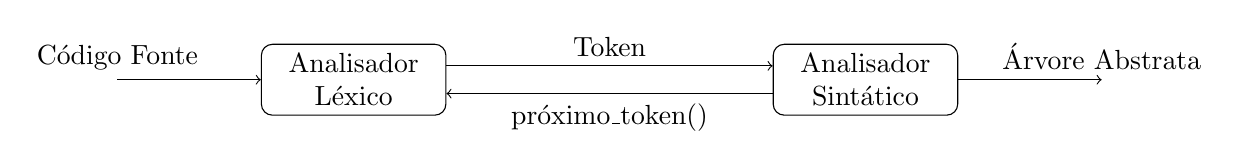
\begin{tikzpicture}[node distance = 3cm, auto]
    % Place nodes
    \node [block]                    (lexico) {Analisador Léxico};
    \node [block, right of = lexico] (sintatico) {Analisador Sintático};
    \coordinate [left of=lexico]     (fonte);
    \coordinate [right of=sintatico] (ast);

    % Draw edges
    \draw[->]    ([yshift=0.5em] lexico.east)       -- ([yshift=0.5em] sintatico.west) node[midway] {Token};
    \draw[->]    ([yshift=-0.5em] sintatico.west)   -- ([yshift=-0.5em] lexico.east)    node[midway] {próximo\_token()};
    \draw[->]    (fonte.west)                       -- (lexico.west)    node[pos=0, above] {Código Fonte};
    \draw[->]    (sintatico.east)                   -- (ast.west)   node[pos=1, above] {Árvore Abstrata};
\end{tikzpicture}
}
\end{center}

\caption{Interações entre um analisador léxico e sintático.}
\label{fig:lexico_sintatico}
\end{figure}

    Primeiro, a análise léxica é responsável por ler o arquivo
de texto contendo o código fonte, e quebrar as palavras em \textit{tokens}, que
serão alimentados para o analisador sintático. Por consequência, ele é capaz de
realizar alguns filtros, \textit{e.g}. ignorar os comentários, identificar constantes
numéricas, eliminar espaços desnecessários, e substituir um \textit{token} por
outro.
Analisadores léxicos também podem ser usados para substituição
de macros, como implementado pelo preprocessador do C
(CPP)\footnote{https://gcc.gnu.org/onlinedocs/cppinternals/Lexer.html}.

Geralmente, os Analisadores Léxicos são implementados utilizando autômatos
por diversos motivos, entre eles sua atrativa complexidade computacional
$O(n)$, onde $n$ é o tamanho da entrada, pela existência de algoritmos
para converter expressões regulares em autômatos \citep{thompson}, e pela
existência de algoritmos para minimização de estados de um autômato
\citep{hopcroft1971n}. Isto possibilita que geradores de analisadores léxicos
como o \texttt{Flex}\footnote{https://www.gnu.org/software/flex/}
sejam bastante eficientes.

    Por fim, o Analisador Sintático entra em cena. O analisador sintático é
responsável por gerar a Árvore de Sintaxe Abstrata (AST), inspecionando a
sequência de \textit{tokens} fornecido pelo Analisador Léxico. Neste processo,
ele certifica-se que o código fonte respeita a gramática da linguagem,
apontando erros caso contrário.

    Analisadores Sintáticos se apoiam nas gramáticas não ambíguas que geram uma
linguagem livre de contexto determinística, isto porque gramáticas mais
poderosas requerem algoritmos computacionalmente mais custosos
\citep{sipser2012}. Existem vários algoritmos para realizar a análise sintática,
mas destacam-se:
\begin{itemize}
    \item LL($k$): Um algoritmo de caráter preditivo, que tenta construir a AST da
        raiz para as folhas. Seu uso é devido a facilidade de codificação e
        mensagens de erros mais informativas para o usuário.

    \item LR($k$): Um algoritmo que tenta construir a AST das folhas para a raiz.
          Sua codificação é mais complicada e as mensagens de erro são mais
          precárias, porém conseguem processar gramáticas mais complexas que
          o LL($k$), conforme proposto por \cite{knuth1965translation}. 
          Outra vantagem interessante é a existência de
          \textit{softwares} como o
          \texttt{Bison}\footnote{https://www.gnu.org/software/bison/}, capaz
          de gerar um analisador LR($1$) a partir da especificação da gramática.
\end{itemize}
	A complexidade destes dois algoritmos é $O(n)$, onde $n$ é o tamanho da entrada.
    Por fim, uma descrição mais detalhada do funcionamento destes algoritmos
pode ser encontrada em \citep{appel2004modern}.

    Uma vez gerada a AST, é possível fazer verificações extras de semântica
relacionada a linguagem de programação, e em seguida essa AST normalmente é
traduzida para uma linguagem intermediária, onde serão feitas otimizações
independentes da linguagem alvo no código. Por fim, o controle é passado
para o \textit{Middle End} do compilador.

\end{subsection}

\begin{subsection}{\textit{Middle End}}

    O \textit{Middle End} é responsável por trabalhar nas uma ou mais
 Linguagens Intermediárias do compilador, com a finalidade de efetuar
otimizações no código e possíveis checagens de erro que possam ser
postergadas até essa fase. Essas linguagens devem ser projetadas
de maneira a capturar a semântica da Linguagem Alvo, na qual o programa original foi
escrito.
Existem várias representações convenientes para a Linguagem Intermediária,
mas destaca-se para fins de otimização 
a \textit{Three-Address Code}, que normalmente é usada em conjunto com
a \textit{Static Single Assignment} (SSA).

\begin{subsubsection}{\textit{Three-Address Code}}


Nesta representação, expressões como $a*x + b$ são
representadas como:
$$ t_1 = a*x$$
\vspace*{-1cm}
$$ t_2 = t_1 + b $$
ou seja, todas as expressões são transformadas em uma sequência de expressões
contendo apenas dois operandos e uma operação de atribuição. Para isso,
novas variáveis são declaradas para conter os valores intermediários
possibilitando também a remoção de sub-expressões em comum.  Também nesta
linguagem, laços e o fluxo de código são transformados em uma sequência de
\texttt{if} e \texttt{goto} para facilitar a construção do grafo de
controle de fluxo, possibilitando análises neste.

Esta representação é demasiada útil por facilitar o processo de alocação
de registradores por representar com fidelidade a maneira de como os processadores
operam instruções aritméticas \citep{lattner2002llvm}.

\end{subsubsection}
\begin{subsubsection}{\textit{Static Single Assignment}}

O \textit{Static Single Assignment} (SSA) é uma linguagem intermediária
onde uma variável é atribuída uma única vez. Sendo assim, toda vez que
uma variável no código original é modificada, na representação SSA é necessário criar uma
nova variável para registrar essa atribuição. Isto facilita diversas
otimizações no controle de fluxo do programa, e possibilita a remoção
de variáveis não utilizadas ou que não serão mais utilizadas em um
trecho de código, processo conhecido como \textit{Liveness Analysis}.

\vspace*{-0.5cm}
Entretanto, isso pode gerar um problema quando essa representação é
    usada em conjunto com um fluxo de execução, como \texttt{if-else}. Considere o código
na Figura \ref{fig:code_normal}. Neste código há dois valores possíveis para
$a$ quando a expressão $u = a*v$ for executada, sendo assim, é necessário
anotar qual versão de $a$ utilizar. A solução é introduzir uma
função $\phi$, que seleciona a variável corretamente utilizando a informação
do arco usado para se chegar no bloco contendo a sentença com a função $\phi$,
conforme ilustrado na Figura \ref{fig:code_ssa_form}.

\begin{figure}[ht]
    \centering
    \begin{subfigure}[b]{0.40\textwidth}

        \begin{lstlisting}[
            language=pseudocode,
            style=pseudocode,
            style=wider,
            functions={},
            specialidentifiers={extern, call},
            ]
            if (condition) then
                a = -1;
            else
                a = 1;
            end
            u = a*v;
        \end{lstlisting}
        \caption{\label{fig:code_normal}}
    \end{subfigure}
    \begin{subfigure}[b]{0.40\textwidth}
        \begin{lstlisting}[
                language=pseudocode,
                style=pseudocode,
                style=wider,
                functions={},
                specialidentifiers={extern, call, PHI},
              ]
            if (condition) then
                $a_1$ = -1;
            else
                $a_2$ = 1;
            end
            $a_3$ = $\phi$($a_1$, $a_2$)
            u = $a_3$*v;
        \end{lstlisting}
        \caption{\label{fig:code_ssa_form}}
\end{subfigure}
\caption{Um programa (a) e sua representação em SSA em (b)}
\end{figure}

Quanto a implementação de SSA em compiladores, \cite{cytron1991efficiently}
discute com detalhes os algoritmos para construir tal representação. Já
\cite{appel2004modern} discute tal representação em alto nível, evidenciando
possíveis otimizações nesta representação.

\end{subsubsection}

\begin{subsubsection}{Otimizações Independente de Arquitetura}

Uma das funcionalidades mais atrativas de um compilador é sua
capacidade de fazer otimizações no código enquanto mantém
a corretude do mesmo, principalmente quando
o alvo é uma linguagem de montagem. Um compilador com essa
funcionalidade é capaz de gerar código que economiza energia
gasta em processamento, poupa esforços de otimização, desenvolvimento,
entre outros.

Considerando o contexto de um compilador capaz de compilar
diversas linguagens para os mais variados alvos, é exatamente
no \textit{Middle End} onde as otimizações independente de
arquitetura devem ocorrer, pois em qualquer outro lugar isto
implicaria em duplicação de código. Sendo assim, boa parte
do esforço de otimização é aplicado aqui.

Como o \textit{Front End} já traduziu todo o código para a linguagem
intermediária, então é perfeitamente possível marcar o inicio de
todas as funções do código. Com isto, é possível particionar o
conjunto das possíveis otimizações em dois conjuntos disjuntos:

\begin{enumerate}
    \item Otimizações \textit{Intra-Procedurais}: Otimizam cada função sem
interagir com as demais funções do programa, por exemplo, Invariante
de Laços, Eliminação de Subexpressão Comum, Propragação de Constantes,
e Eliminação de Código Morto.

    \item Otimizações \textit{Inter-Procedurais}: Procuram observar o programa
como um todo, observando as interações de cada função com as demais
funções do programa.
\end{enumerate}
Essa distinção é útil pois não há dependência entre as funções
ao aplicar uma otimização \textit{Intra-Procedural}, e portanto as
funções podem ser processadas em paralelo.
Diversas otimizações
clássicas como Invariante de Laços, Propagação de Constantes,
Eliminação de Redundância, Eliminação de Subexpressão Comum,
Propagação de Constantes, e Eliminação de Código Morto são
classificadas como tal, suportando o argumento de paralelização.

Já esse argumenton não pode
ser afirmado para as otimizações \textit{Inter-Procedurais}, pela
própria definição. 
Otimizações \textit{Inter-Procedurais} são normalmente aplicadas
utilizando algoritmos em grafos:
Cada rotina é representado como um vértice, e existe um arco de $f$
à $g$ se $f$ chama $g$ em seu corpo, conforme ilustrado na Figura
\ref{fig:call_graph}. Construir tal grafo pode ser
um desafio dependendo da linguagem de programação, principalmente
quando se utiliza orientação a objetos devido a possibilidade de
sobrescrita de métodos. Por fim, mais detalhes a respeito dos 
algoritmos referentes a essas otimizações são discutidos por
\cite{khedker2009data}.

\begin{figure}[ht]
\centering
  \begin{subfigure}[b]{0.40\textwidth}
    \tikzstyle{line} = [draw, -latex]
    \tikzstyle{node} = [draw, circle]
    \begin{center}
    \scalebox{0.8}{
    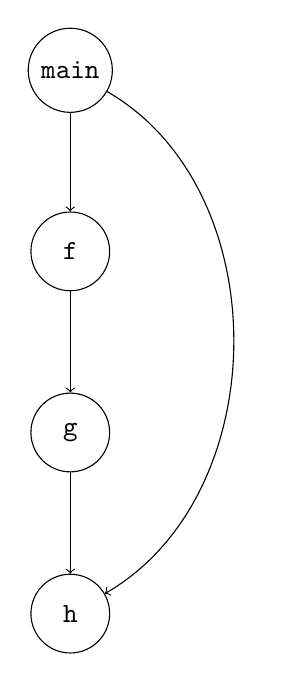
\begin{tikzpicture}[node distance = 2.3cm, minimum height = 1cm, auto]
        % Place nodes
        \node [node]                    (main) {\texttt{main}};
        \node [node, below of = main]        (f) {\texttt{f}};
        \node [node, below of = f]           (g) {\texttt{g}};
        \node [node, below of = g]           (h) {\texttt{h}};

        % Draw edges
        \draw[->]    (main)           -- (f);
        \draw[->]    (f)              -- (g);
        \draw[->]    (g)              -- (h);
        \draw[->]    (main)      to [out=-30,in=30] (h);
    \end{tikzpicture}
    }
    \end{center}
    \label{fig:call_graph}
  \end{subfigure}
  \begin{subfigure}[b]{0.40\textwidth}
      \begin{lstlisting}[
        language=pseudocode,
        style=pseudocode,
        style=wider,
        functions={},
        specialidentifiers={extern, call},
      ]
        extern function g,h

        function f()
            call $g$
            call $h$
        end

        function main()
            call $f$
            call $h$
        end
      \end{lstlisting}
  \end{subfigure}
  \caption{Um programa e seu respectivo grafo de chamada de funções}
  \label{fig:call_graph}
\end{figure}


    Após todo esse processo de otimização, o código nesta linguagem ainda
pode ainda sofrer transformações para outras Linguagens
Intermediárias para algo que seja mais próximo do
\textit{hardware}-alvo, no caso da compilação ter como alvo código de máquina.
Finalmente, após essa sequência de transformações, o controle é
passado ao \textit{Back End} do compilador, onde ele será transformado na
Linguagem Alvo.

\end{subsubsection}

\end{subsection}

\begin{subsection}{\textit{Back End}}
    O \textit{Back End} é responsável pela geração do código final na
Linguagem Alvo, além otimizações dependentes
de arquitetura. Sendo assim, ele também deve efetuar otimizações referente
a  seleção de instruções mais eficazes e alocação registradores
da melhor maneira possível para as variáveis do programa, caso a linguagem alvo
seja a Linguagem de Montagem.

    Existem diversas técnicas para selecionar instruções. Uma estratégia possível
é  utilizar uma abordagem de substituição de macros, onde as instruções são substituídas
observando localmente cada linha de código da Linguagem Intermediária. Esta estratégia
tem a vantagem de realizar uma tradução rápida e de fácil implementação, mas que gera
código ineficiente. 

    Outra maneiras incluem identificar padrões a partir de uma árvore
construída, e selecionar a construção que minimiza uma função custo, seja através de uma
heurística, ou usando \textit{Programação Dinâmica}. 

	Também é possível implementar tal tradução utilizando as mesmas técnicas de
análise léxica e sintática empregados no \textit{Front End}, desde que a
Linguagem Intermediária tenha sido projetada considerando tal fato, conforme
sugerido por \cite{glanville1978}. 

Por fim, uma discussão mais detalhada sobre
as técnicas de geração de código de máquina é discutida por
\citep{blindell2016instruction}. Além disso, para 
 adicionar suporte a uma nova arquitetura ou linguagem
alvo, basta implementar um novo \textit{Back End}, aproveitando todo
o código já implementado nas etapas anteriores.
\end{subsection}


\end{section}

\begin{section}{Computação Paralela}

\end{section}



\begin{section}{O compilador GCC}

%    Para realizar otimizações considerando as interações entre as rotinas,
%é utilizado um grafo de chamada de funções (\texttt{cgraphs}). Aqui as rotinas são
%representadas como um vértice no grafo, e existe um arco de $f$ à $g$
%quando há uma chamada de $g$ a partir de $f$. Dependendo da linguagem de
%programação utilizada, construir tais grafos pode ser uma tarefa simples pois
%as chamadas são especificadas estaticamente, como é o caso de Fortran; mas
%isto pode se tornar algo extremamente complexo quando orientação à objetos é
%empregada, pois é possível sobrescrever métodos.
%
%    Os grafos de chamadas de funções permitem otimizações que eliminem chamadas
%de funções, economizando assim o custo da chamada, e ainda permitem com que as
%funções sejam emitidas por ordem de proximidade, evitando com que o salto no
%fluxo de execução seja demasiado longo, o que implicaria em \textit{cache miss}.
%Também é possível propagar informações a respeito de outras funções, por exemplo
%propagar que uma certa função não altera um estado global ou interno desta
%(e.g. imprimir na tela, alterar um objeto), e em seguida calcular o resultado
%desta em tempo de compilação e remover sua chamada. Isto permite binários menores
%e código mais rápido, pois evita a necessidade de computar valores em tempo de
%execução.
%

%Um exemplo é o \textit{Register Transfer Language} (RTL) onde o código é
%representado como uma sequência de instruções em uma máquina de infinitos
%registradores. 

\begin{subsection}{GNU Toolchain e as etapas da compilação}

\begin{figure}
\tikzstyle{block} = [rectangle, draw, fill=white,
    text width=6em, text centered, rounded corners, node distance=6.5cm, auto, minimum height=2em]
\tikzstyle{line} = [draw, -latex]
\tikzstyle{cloud} = [draw, ellipse,fill=white, node distance=2cm,
    minimum height=2em]
\begin{center}
\scalebox{0.7}{
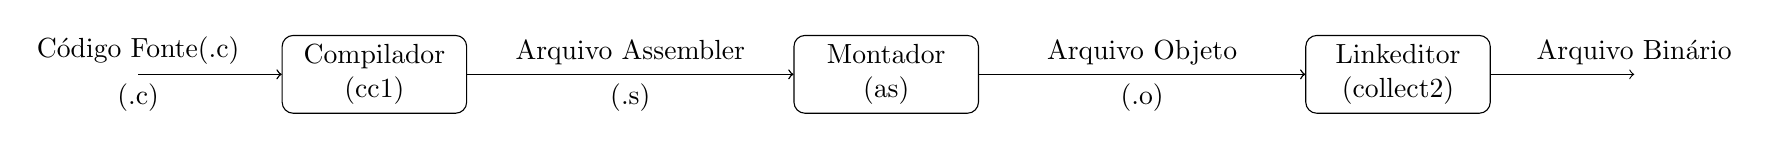
\begin{tikzpicture}[node distance = 3cm, auto]
    % Place nodes
    \node [block]                      (cc1) {Compilador \\ (cc1)};
    \node [block, right of = cc1]      (as) {Montador\\(as)};
    \node [block, right of = as]       (collect2) {Linkeditor\\(collect2)};
    \coordinate [left of=cc1]          (fonte);
    \coordinate [right of=collect2]    (bin);

    % Draw edges
    \draw[->]    (cc1.east)          -- (as.west)       node[midway, above] {Arquivo Assembler};
    \draw[->]    (cc1.east)          -- (as.west)       node[midway, below] {(.s)};
    \draw[->]    (as.east)           -- (collect2.west) node[midway, above] {Arquivo Objeto};
    \draw[->]    (as.east)           -- (collect2.west) node[midway, below] {(.o)};
    \draw[->]    (fonte.west)        -- (cc1.west)      node[pos=0, above] {Código Fonte\\ (.c)};
    \draw[->]    (fonte.west)        -- (cc1.west)      node[pos=0, below] {(.c)};
    \draw[->]    (collect2.east)     -- (bin.west)      node[pos=1, above] {Arquivo Binário};
\end{tikzpicture}
}
\end{center}

\caption{Etapas de Compilação.}
\label{fig:gnu_toolchain}
\end{figure}

\end{subsection}

\end{section}
